\section{GARCH 的估计、诊断与扩展}
\label{sec:11-Mathematical-Statistics/10-GARCH-and-Volatility/03}

第一次动手估 GARCH，多半会在三个地方卡住。似然函数里 \(\sigma_t^2\) 是递归出来的，没有闭式；递归得有个起点，而 \(\sigma_0^2\) 谁也没给；优化跑完一看，\(\hat\beta=0.9997\) 死死贴在约束边界上。这些都不是软件的问题，而是这个模型的结构决定的。这一节把估计、诊断、扩展三件事串起来，最后回答一个在实践中被反复搞混的问题：拟合好的 GARCH 到底能预测什么。

\subsection{条件似然是一条递归}

似然的构造靠链式分解。联合密度可以拆成一串条件密度的乘积，

\[
p(\varepsilon_1,\dots,\varepsilon_T;\theta)=\prod_{t=1}^{T}p(\varepsilon_t\given\mathcal F_{t-1};\theta),
\]

而 GARCH 恰好把每个条件密度都写清楚了：给定 \(\mathcal F_{t-1}\)，\(\varepsilon_t\) 服从均值零、方差 \(\sigma_t^2(\theta)\) 的分布。若创新取正态，对数似然是

\[
\ell(\theta)=-\frac12\sum_{t=1}^{T}\left(\log 2\pi+\log\sigma_t^2(\theta)+\frac{\varepsilon_t^2}{\sigma_t^2(\theta)}\right),
\qquad \theta=(\omega,\alpha,\beta).
\]

这个式子和\hyperref[sec:11-Mathematical-Statistics/02-Point-Estimation/03]{``最大似然选择最能解释数据的参数''}里的一般框架完全同构，唯一的特别之处在于 \(\sigma_t^2(\theta)\) 不是参数的显式函数，而要靠 \(\sigma_t^2=\omega+\alpha\varepsilon_{t-1}^2+\beta\sigma_{t-1}^2\) 从头递推一遍。每次优化器换一组 \(\theta\)，都要把整条序列重扫一次。

递归的起点按惯例取 \(\sigma_1^2=\hat\omega/(1-\hat\alpha-\hat\beta)\) 或者干脆用样本方差。这个选择的影响以 \(\beta^{\,t}\) 衰减，样本长时几乎不可见；但样本只有两三百期、且 \(\beta\) 接近一时，它能实实在在地挪动估计值。遇到结论对初始化敏感的情况，通常说明数据量不够支撑这个参数化，而不是初始化方案该换。

约束是三条：\(\omega>0\)，\(\alpha,\beta\ge0\)，\(\alpha+\beta<1\)。数值上更稳的做法是重参数化到无约束空间再优化，比如令 \(\omega=e^{u}\)，用 logistic 变换把 \((\alpha,\beta)\) 映到单纯形内部。这样优化器不会在边界上反复撞墙，代价是标准误要用 delta 方法换算回原参数。

还有一条实践中很重要的退路。即使 \(z_t\) 并不服从正态，最大化上面这个正态似然得到的 \(\hat\theta\) 在适当矩条件下仍然相合——因为正态似然的一阶条件本质上只利用了前两阶条件矩，而这两阶正是模型说对了的部分。这就是拟极大似然（QMLE）。它的代价出在标准误上：信息矩阵等式不再成立，必须用 sandwich 形式的稳健协方差，否则参数显著性会被系统性高估。

\subsection{诊断的对象是标准化残差，不是残差}

拟合完成后，把残差除以它自己的条件标准差：

\[
\hat z_t=\frac{\varepsilon_t}{\hat\sigma_t}.
\]

模型若说对了，\(\hat z_t\) 就该是独立同分布、均值零、方差一的序列。所有诊断都对着它做，而不是对着 \(\varepsilon_t\) 做——\(\varepsilon_t\) 本来就该是异方差的，检验它没有意义。

三件事值得逐一确认。第一，\(\hat z_t\) 的自相关应当消失，否则条件均值那一层还有结构没抓干净。第二，\(\hat z_t^2\) 的自相关也应当消失，这一步直接对应\hyperref[sec:11-Mathematical-Statistics/10-GARCH-and-Volatility/01]{``条件异方差的统计特征''}里立下的那个动作：拟合前用它发现问题，拟合后用它确认问题已经解决。若 \(\hat z_t^2\) 仍显著自相关，说明 GARCH(1,1) 的记忆结构不够，该提阶或者换设定。第三，\(\hat z_t\) 的分布形状要看 QQ 图；若两端明显偏离正态直线，说明厚尾没有被条件方差吸收干净。

要注意 Ljung--Box 统计量的自由度问题：\(\hat z_t\) 是估计出来的，不是观测到的，检验统计量的零分布会因参数估计而改变，直接查表容易得到偏乐观的 \(p\) 值。稳妥的做法是把它当作定性信号，或者用自助法重算临界值。

\subsection{正负冲击的影响可以不对称}

标准 GARCH 里 \(\varepsilon_{t-1}\) 只以平方的形式进入，符号被抹掉了：跌 \(2\%\) 和涨 \(2\%\) 对明天的波动预测贡献一模一样。数据往往不同意这一点。股票收益率里负冲击推高波动更多，早期的解释是价格下跌抬高了财务杠杆，名字就此叫作杠杆效应；而在服务指标上，同样的形态来自另一处——错误率突然上升会触发重试、降级、人工介入，这些动作本身制造更多抖动，而错误率下降不会。

GJR-GARCH 用一个指示函数把这层不对称加进来：

\[
\sigma_t^2=\omega+\alpha\varepsilon_{t-1}^2+\gamma\ind\set{\varepsilon_{t-1}<0}\varepsilon_{t-1}^2+\beta\sigma_{t-1}^2 .
\]

\(\gamma>0\) 表示负冲击多出一份影响。检验杠杆效应就退化成检验 \(\gamma=0\)，一个标准的参数检验。EGARCH 走另一条路，直接建模对数方差：

\[
\log\sigma_t^2=\omega+\alpha\frac{\abs{\varepsilon_{t-1}}}{\sigma_{t-1}}+\gamma\frac{\varepsilon_{t-1}}{\sigma_{t-1}}+\beta\log\sigma_{t-1}^2 ,
\]

其中 \(\gamma<0\) 对应杠杆效应。用对数的好处是 \(\sigma_t^2\) 自动为正，参数不需要非负约束，优化空间干净很多。

把这两类模型的差别画出来最直观。固定 \(\sigma_{t-1}\)，看下一期条件方差怎样随本期冲击变化，这条曲线叫新闻冲击曲线。

\begin{center}
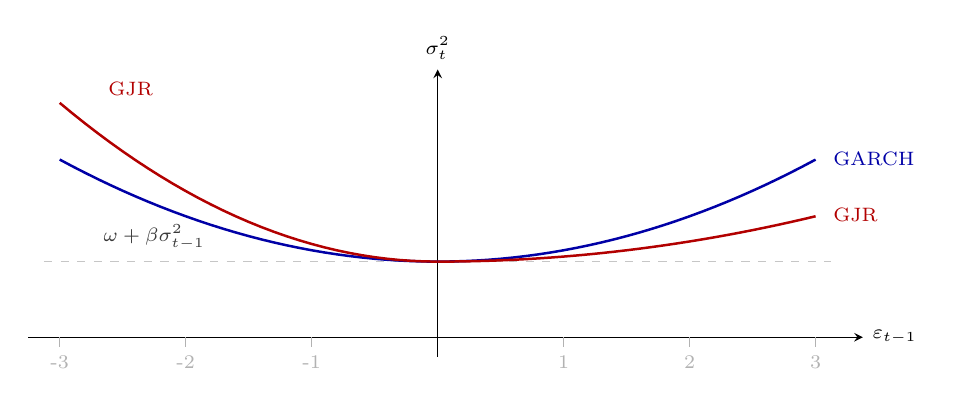
\begin{tikzpicture}[>=stealth]
\draw[->] (-5.2,0) -- (5.4,0) node[right,font=\scriptsize] {\(\varepsilon_{t-1}\)};
\draw[->] (0,-0.25) -- (0,3.4) node[above,font=\scriptsize] {\(\sigma_t^2\)};
\foreach \x in {-3,-2,-1,1,2,3}
  \draw[gray!60] (1.6*\x,0) -- (1.6*\x,-0.12) node[below,font=\scriptsize] {\x};
\draw[gray!45,dashed] (-5,0.96) -- (5,0.96);
\node[font=\scriptsize,gray!45!black,above] at (-3.6,0.99) {\(\omega+\beta\sigma_{t-1}^2\)};
% 对称 GARCH
\draw[blue!65!black,line width=0.9pt,domain=-3:3,samples=61]
  plot ({1.6*\x},{1.6*(0.6+0.09*\x*\x)});
% GJR：负半轴更陡
\draw[red!70!black,line width=0.9pt,domain=-3:0,samples=31]
  plot ({1.6*\x},{1.6*(0.6+0.14*\x*\x)});
\draw[red!70!black,line width=0.9pt,domain=0:3,samples=31]
  plot ({1.6*\x},{1.6*(0.6+0.04*\x*\x)});
\node[font=\scriptsize,blue!65!black,right] at (4.9,2.26) {GARCH};
\node[font=\scriptsize,red!70!black] at (-3.9,3.15) {GJR};
\node[font=\scriptsize,red!70!black,right] at (4.9,1.55) {GJR};
\end{tikzpicture}
\end{center}

\emph{新闻冲击曲线：对称 GARCH 是一条正抛物线，GJR 在负半轴更陡、正半轴更平。}

图里两条曲线在原点附近几乎重合，差别全在两翼。这意味着在平静期两个模型给出的预测差不多，分歧只在冲击较大时出现——而那正是波动预测被真正用到的时候。这也是为什么杠杆效应不该按``模型精度提升零点几个百分点''来评估，它改变的是尾部。

\subsection{厚尾要放在新息里，而不是靠条件方差硬撑}

条件异方差本身就能生成无条件厚尾，本单元第一节算过 ARCH(1) 的峰度。但对不少序列，把条件方差建到最好之后，\(\hat z_t\) 的 QQ 图两端仍然翘出去。这说明新息 \(z_t\) 自己就不是正态的。

处理办法是把 \(z_t\) 换成标准化的 Student-\(t\)，多估一个自由度 \(\nu\)。\(\nu\to\infty\) 退回正态，实际数据常落在 \(4\) 到 \(10\) 之间。这个替换对参数点估计影响不大，对分位数影响相当大。取 \(\nu=5\) 的标准化 \(t\)：\(99\%\) 分位数是 \(2.61\)，正态是 \(2.33\)；到了 \(99.9\%\) 分位数，两者是 \(4.57\) 与 \(3.09\)。越往尾部走差距越大，而风险度量恰恰住在尾部。用正态新息去算 \(99.9\%\) 的风险敞口，会系统性地低估三分之一左右。

\begin{remark}
用 QMLE 时可以不管分布假设错设，因为你只要参数相合。一旦要输出分位数、风险价值或者预测区间，分布假设就重新变成第一位的了——那时 \(\hat\sigma_t\) 只是刻度，形状由 \(z_t\) 的分布决定。
\end{remark}

\subsection{GARCH 预测幅度，不预测方向}

这是整个单元最容易被误用的地方。模型的均值方程从头到尾只有一句 \(\E[\varepsilon_t\given\mathcal F_{t-1}]=0\)。无论 \(\hat\sigma_t\) 怎么变化，条件均值预测始终是零；波动率预测上升，意味着明天的分布更宽，不意味着它会往下走。按\hyperref[sec:05-Probability/04-Expectation-and-Moments/04]{``条件期望是利用信息的最佳预测''}的说法，GARCH 改进的是二阶条件矩，一阶条件矩它压根没碰。

把这句话摊开，就得到一份用途清单和一份禁区清单。可以做的是：算条件分位数，\(\text{VaR}_{t}(p)=\hat\sigma_t\,q_p\)，其中 \(q_p\) 是新息分布的分位数；给预测区间定宽度，让区间在高波动期自动变宽，覆盖率回到名义水平；把\hyperref[sec:11-Mathematical-Statistics/10-GARCH-and-Volatility/01]{``条件异方差的统计特征''}里那个固定阈值换成 \(\abs{\varepsilon_t}>c\,\hat\sigma_t\)，误报率就不再随波动期漂移；做容量规划时按预测的波动而不是预测的均值留余量，这与\hyperref[sec:11-Mathematical-Statistics/07-Statistical-Decision-and-Reliable-Prediction/06]{``拒绝预测与容量约束把概率变成行动''}里把概率翻译成行动的思路是同一条。

不能做的是：拿 \(\hat\sigma_t\) 上升当看空信号，拿它下降当看多信号，或者把波动率预测直接接进一个方向性的下单逻辑。真要预测方向，得另外写一个条件均值方程，用 ARMA、回归或者别的什么，然后让 GARCH 负责这个均值方程的残差。两层是分开的，一层管去哪儿，一层管有多颠。

\subsection{往外走的几个方向}

GARCH(1,1) 是起点而不是终点，几个常见的延伸都对应着某条假设被数据推翻。平方序列的自相关若按幂律而非几何衰减，几何加权就不够了，FIGARCH 用分数差分补上这段长记忆。参数若在样本中途换了值，单一模型会把结构突变误读成近似单位根，Markov 转换 GARCH 让参数在若干状态间跳。有日内数据可用时，已实现波动率携带的信息远多于日频收益率平方，HAR 之类的模型直接对它建模。要同时管多个序列的协方差矩阵，则进入 DCC 或 BEKK 的领域，那里主要的困难变成了如何在维数增长时保持矩阵正定。

这些扩展看起来很散，共同的骨架其实一直没变：一个可测于过去的方差方程，一个标准化到均值零方差一的新息，以及一次靠条件似然完成的估计。诊断的动作也没变——把标准化残差拿出来，看它还剩多少结构。哪一天这个残差干净了，模型就到位了；只要它还不干净，无论加多少花样，欠的都是同一笔账。
